\section{Statistical Analysis of the Latent Material Description}
\label{app:latent_analysis}

We complement the qualitative latent space visualizations in Appendix~\ref{app:latent_vis} with two quantitative analyses of the latent material description $\mathbf{r}$. Appendix~\ref{app:r_convergence} investigates how $\mathbf{r}$ behaves within a task as the number of context trajectories grows, and Appendix~\ref{app:rsa} investigates whether $\mathbf{r}$ preserves the structure of the physical parameters across tasks.

\subsection{Convergence with Context Size}
\label{app:r_convergence}

Ideally, the latent material description converges to a fixed descriptor of the task, and additional context trajectories reduce its variance at a rate comparable to averaging independent observations.

\paragraph{Setup.}
Each test task consists of $N$ trajectories that share the same physical properties, with $N=16$ for \texttt{Deforming Block} and \texttt{Sheet Deformation} and $N=10$ for \texttt{Bending Beam} and \texttt{Trampoline}. For every context size $C \in \{1, \dots, 8\}$, we sample up to $250$ context sets $S_C$ of $C$ trajectories without replacement, or use all possible sets if fewer exist, and encode each set into its aggregated latent representation $\mathbf{r}(S_C)$. As the latent space has no natural scale, we standardize each of its dimensions by its mean and standard deviation over all latent vectors of an environment. We then measure the variance of the standardized representations $\tilde{\mathbf{r}}$ across the sampled context sets of a task as
\begin{equation*}
    \mathrm{Var}(C) = \frac{1}{M_C - 1} \sum_{m=1}^{M_C} \bigl\| \tilde{\mathbf{r}}(S_C^{(m)}) - \bar{\mathbf{r}}_C \bigr\|^2 ,
\end{equation*}
where $M_C$ is the number of sampled context sets and $\bar{\mathbf{r}}_C$ their mean representation.

\paragraph{Variance model.}
For a plain average of $C$ independent samples, the variance decreases as $C^{-1}$. Since our context sets are drawn without replacement from a finite pool of $N$ trajectories, the variance across context sets is additionally reduced by the finite population correction $(N-C)/(N-1)$, which becomes substantial for large $C$ relative to $N$. We therefore fit the model
\begin{equation*}
    \mathrm{Var}(C) = \sigma^2 \, C^{-\beta_r} \, \frac{N - C}{N - 1}
\end{equation*}
to each task individually via least squares in log space. Under this model, $\beta_r = 1$ corresponds exactly to averaging independent trajectory embeddings. Values $\beta_r < 1$ indicate a slower variance reduction, for example due to redundant context trajectories, while $\beta_r > 1$ indicates that the aggregation reduces the variance faster than a plain average. Note that the learned softmax aggregation of \gls{peach} is not a plain average, so the model serves as a reference rather than an exact description.

\paragraph{Results.}
Figure~\ref{fig:variance_shrinkage} shows the normalized variance $\mathrm{Var}(C)/\mathrm{Var}(1)$ for all test tasks, and Table~\ref{tab:beta_r} reports the fitted exponents. In all environments, the variance of $\mathbf{r}$ decreases consistently with the context size, and the curves of individual tasks closely follow the median, indicating that the latent description converges for all tasks rather than only on average. For \texttt{Deforming Block}, \texttt{Sheet Deformation}, and \texttt{Bending Beam}, the median exponents lie close to $\beta_r=1$, i.e., the aggregated representation behaves like an average over independent observations of the task. \texttt{Bending Beam} shows the largest spread across tasks, which we attribute to its three varying material parameters that are not equally observable in every trajectory. For \texttt{Trampoline}, the variance decreases more slowly with $\beta_r = 0.73$. Here, the trajectories of a task only differ in the drop position and height of the ball, so additional context trajectories provide partially redundant information about the material. Overall, the consistent variance reduction matches the steady improvement of the simulation accuracy with increasing context size reported in Appendix~\ref{app:quant}.

\begin{figure}[t]
    \centering
    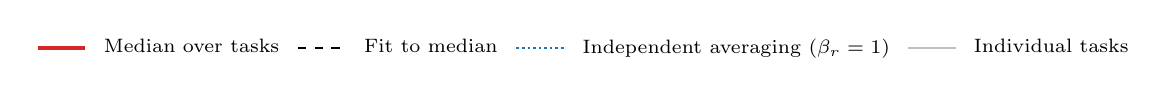
\begin{tikzpicture}
        \tikzstyle{every node}=[font=\scriptsize]
        \definecolor{tabblue}{RGB}{31, 119, 180}
\definecolor{taborange}{RGB}{255, 127, 14}
\definecolor{tabgreen}{RGB}{44, 160, 44}
\definecolor{tabred}{RGB}{214, 39, 40}
\definecolor{tabpurple}{RGB}{148, 103, 189}
\definecolor{tabbrown}{RGB}{140, 86, 75}
\definecolor{tabpink}{RGB}{227, 119, 194}
\definecolor{tabgray}{RGB}{127, 127, 127}
\definecolor{tabolive}{RGB}{188, 189, 34}
\definecolor{tabcyan}{RGB}{23, 190, 207}
\definecolor{ForestGreen}{RGB}{34, 139, 34}

        \begin{axis}[%
            hide axis,
            xmin=10,
            xmax=50,
            ymin=0,
            ymax=0.1,
            legend style={
                draw=none,
                legend cell align=left,
                legend columns=4,
                column sep=1ex,
            }
        ]

        \addlegendimage{line legend, tabred, line width=1.2pt}
        \addlegendentry{Median over tasks}

        \addlegendimage{line legend, black, dashed, line width=1pt}
        \addlegendentry{Fit to median}

        \addlegendimage{line legend, tabblue, densely dotted, line width=1pt}
        \addlegendentry{Independent averaging ($\beta_r=1$)}

        \addlegendimage{line legend, black!25, line width=0.6pt}
        \addlegendentry{Individual tasks}

        \end{axis}
    \end{tikzpicture}\\[2pt]
    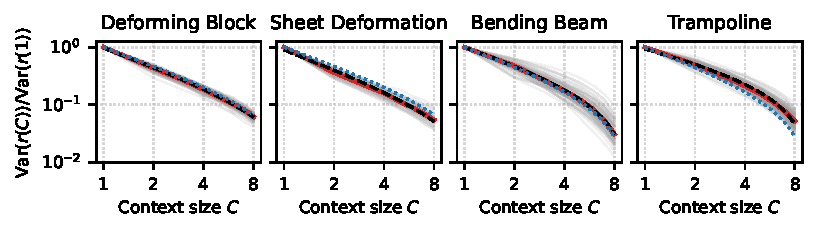
\includegraphics[width=\textwidth]{figures/variance_shrinkage.pdf}
    \caption{Variance of the latent material description $\mathbf{r}$ across context sets of size $C$, normalized per task by its variance at $C=1$. The dashed line shows the fitted power law with finite population correction on the median curve, and the dotted line shows the expected decrease for averaging independent samples.}
    \label{fig:variance_shrinkage}
\end{figure}

\begin{table}[t]
    \centering
    \caption{Fitted variance exponent $\beta_r$ of the latent material description. We report the median over all test tasks, with the interquartile range in brackets. $\beta_r = 1$ corresponds to averaging independent samples.}
    \label{tab:beta_r}
    \begin{tabular}{lcccc}
    \toprule
     & \texttt{Deforming Block} & \texttt{Sheet Deformation} & \texttt{Bending Beam} & \texttt{Trampoline} \\
    \midrule
    $\beta_r$ & $1.03$ \small{$[0.99, 1.06]$} & $1.08$ \small{$[1.04, 1.13]$} & $0.96$ \small{$[0.77, 1.07]$} & $0.73$ \small{$[0.64, 0.83]$} \\
    \bottomrule
    \end{tabular}
\end{table}

\subsection{Correspondence to Physical Parameters}
\label{app:rsa}

A useful latent material description should organize tasks according to their physical properties, i.e., tasks with similar parameters should be encoded close to each other. We test this with a representational similarity analysis~\citep{kriegeskorte2008rsa} across all test tasks of an environment.

\paragraph{Setup.}
For each test task, we estimate its latent description as the mean of the standardized representations $\tilde{\mathbf{r}}(S_C)$ over all sampled context sets of the largest context size $C=8$, which yields the most converged estimate. We normalize each ground-truth physical parameter by its standard deviation across the test tasks of an environment, so that all parameters contribute equally. We then compute two matrices of pairwise Euclidean distances between tasks, one in the space of physical parameters $\rho$ and one in the latent space $\mathbf{r}$, and measure their correspondence via the Spearman correlation between their upper triangles. Since every task contributes to many pairs, the pairs are not independent, and we assess significance with a Mantel test~\citep{mantel1967detection} that permutes the task labels of one matrix $9999$ times. As a complementary local measure, we report the neighbor agreement, i.e., the fraction of each task's $3$ nearest neighbors in $\rho$ that are also among its $3$ nearest neighbors in $\mathbf{r}$, averaged over all tasks.

Additionally, we estimate the effective dimensionality of the latent descriptions across tasks via the participation ratio
\begin{equation*}
    \mathrm{PR} = \frac{\bigl(\sum_i \lambda_i\bigr)^2}{\sum_i \lambda_i^2} ,
\end{equation*}
where $\lambda_i$ are the eigenvalues of the covariance matrix of the task-level latent descriptions. The participation ratio ranges from $1$, if all variance lies along a single direction, to the full latent dimension, if the variance is spread evenly. We compute it on the mean-centered but otherwise unstandardized representations, since standardizing each dimension would equalize the variance of uninformative directions and thereby inflate the estimate.

\paragraph{Results.}
Figure~\ref{fig:rsa_distances} shows the pairwise task distances in both spaces, and Table~\ref{tab:rsa} summarizes the statistics. For the single-parameter environments \texttt{Deforming Block} and \texttt{Sheet Deformation}, the distances correspond almost perfectly with Spearman correlations of $0.97$ and $0.96$. The relationship is monotone but concave, as distances in $\mathbf{r}$ saturate for very different materials, which the rank-based correlation does not penalize. For \texttt{Bending Beam} and \texttt{Trampoline}, the correlations of $0.64$ and $0.60$ are lower but still highly significant, and the neighbor agreement is roughly ten times above chance level in all environments. We attribute the larger spread in these environments to parameters with little influence on the observed dynamics. Since all parameters contribute equally to the distance in $\rho$, tasks that differ mainly in such a parameter appear far apart in $\rho$ but behave almost identically, and are thus correctly encoded close to each other in $\mathbf{r}$.

The participation ratio supports this interpretation. For the single-parameter environments, it lies close to $1$, i.e., the latent descriptions essentially vary along a single direction. For \texttt{Trampoline}, the participation ratio of $2.78$ is smaller than the five varying parameters. As shown in Figure~\ref{fig:latents_appendix}, the behavior of this scene is mainly governed by the loading ratio, which combines the ball mass, the Young's modulus, and the sheet thickness into a single quantity, and by the relaxation time, while the shear relaxation ratio has little visible effect. For \texttt{Bending Beam}, the participation ratio of $4.15$ exceeds the three varying material parameters. This is consistent with our interpretation that the latent description does not merely encode the material parameters, but an effective behavior that also compensates for approximation errors of the learned simulator, which need not align with the directions of the individual parameters.

\begin{figure}[t]
    \centering
    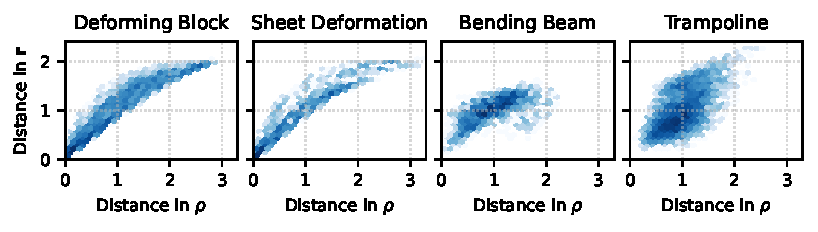
\includegraphics[width=\textwidth]{figures/rsa_distances.pdf}
    \caption{Pairwise distances between test tasks in the space of ground-truth physical parameters $\rho$ and in the latent space $\mathbf{r}$, both normalized by their mean. Each hexagon counts task pairs on a logarithmic color scale. Tasks with similar physical parameters are consistently encoded close to each other, while the larger spread in \texttt{Bending Beam} and \texttt{Trampoline} stems from parameters with little influence on the observed dynamics.}
    \label{fig:rsa_distances}
\end{figure}

\begin{table}[t]
    \centering
    \caption{Correspondence between the latent material description $\mathbf{r}$ and the ground-truth physical parameters $\rho$ across test tasks. Spearman correlations are computed between pairwise task distances and tested with a Mantel test using $9999$ permutations, all with $p < 10^{-3}$. Neighbor agreement is the fraction of each task's $3$ nearest neighbors in $\rho$ that are also among its $3$ nearest neighbors in $\mathbf{r}$, with the chance level in brackets.}
    \label{tab:rsa}
    \begin{tabular}{lcccc}
    \toprule
     & \shortstack{\texttt{Deforming}\\\texttt{Block}} & \shortstack{\texttt{Sheet}\\\texttt{Deformation}} & \shortstack{\texttt{Bending}\\\texttt{Beam}} & \texttt{Trampoline} \\
    \midrule
    Test tasks & $100$ & $50$ & $60$ & $100$ \\
    Spearman correlation & $0.97$ & $0.96$ & $0.64$ & $0.60$ \\
    Neighbor agreement & $0.69$ \small{$[0.03]$} & $0.85$ \small{$[0.06]$} & $0.54$ \small{$[0.05]$} & $0.31$ \small{$[0.03]$} \\
    Varying parameters & $1$ & $1$ & $3$ & $5$ \\
    Participation ratio & $1.56$ & $1.49$ & $4.15$ & $2.78$ \\
    \bottomrule
    \end{tabular}
\end{table}